\section{Arquitectura Objetivo}
La Figura~\ref{fig:arquitectura-objetivo} muestra la composición de contenedores y servicios que sostiene la arquitectura objetivo.
\IfFileExists{figures/generated/01_arquitectura_objetivo.pdf}{
\begin{figure}[htbp]
  \centering
  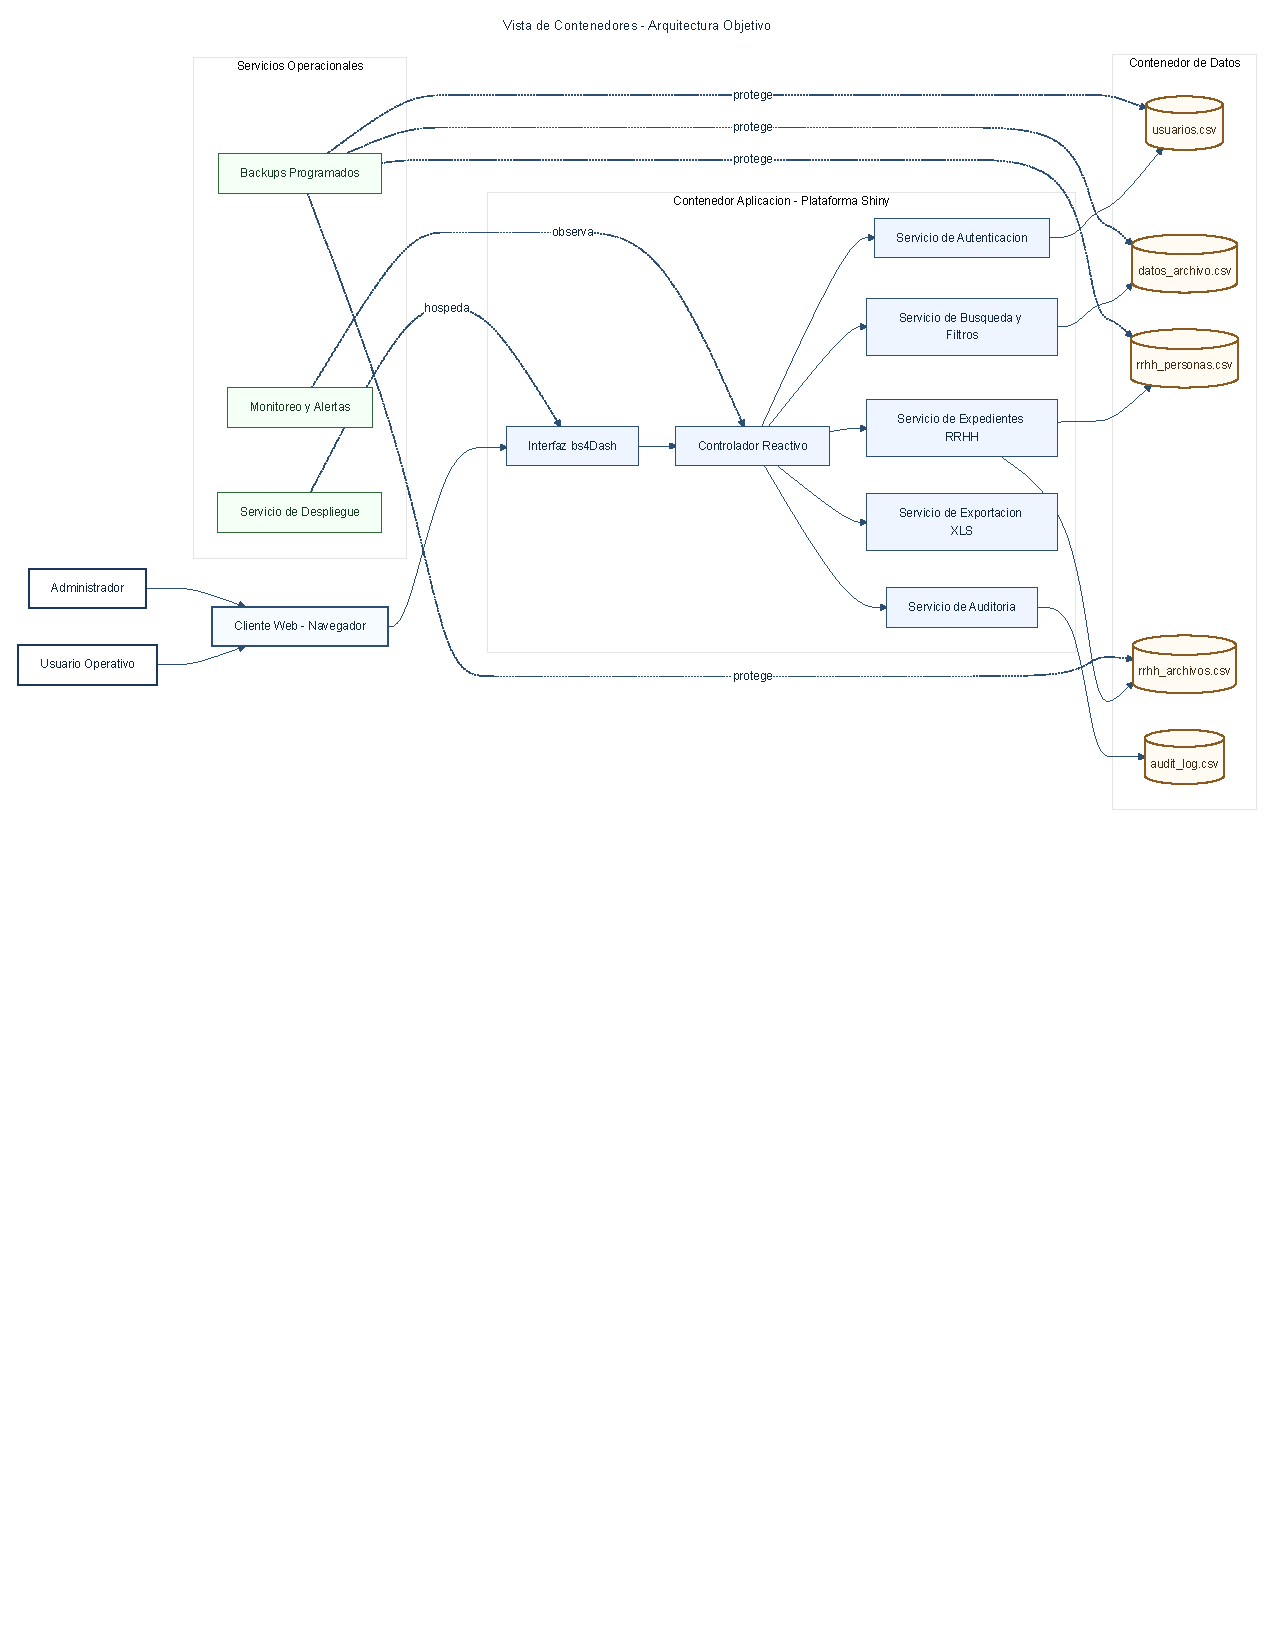
\includegraphics[width=\textwidth]{figures/generated/01_arquitectura_objetivo.pdf}
  \caption{Vista de contenedores de la arquitectura objetivo}
  \label{fig:arquitectura-objetivo}
\end{figure}
}{
\textit{Diagrama pendiente de exportacion: 01\_arquitectura\_objetivo.pdf}
}

\section{Flujo de Autenticacion}
La Figura~\ref{fig:flujo-autenticacion} presenta el recorrido de autenticación y control de acceso entre los componentes del sistema.
\IfFileExists{figures/generated/02_flujo_autenticacion.pdf}{
\begin{figure}[htbp]
  \centering
  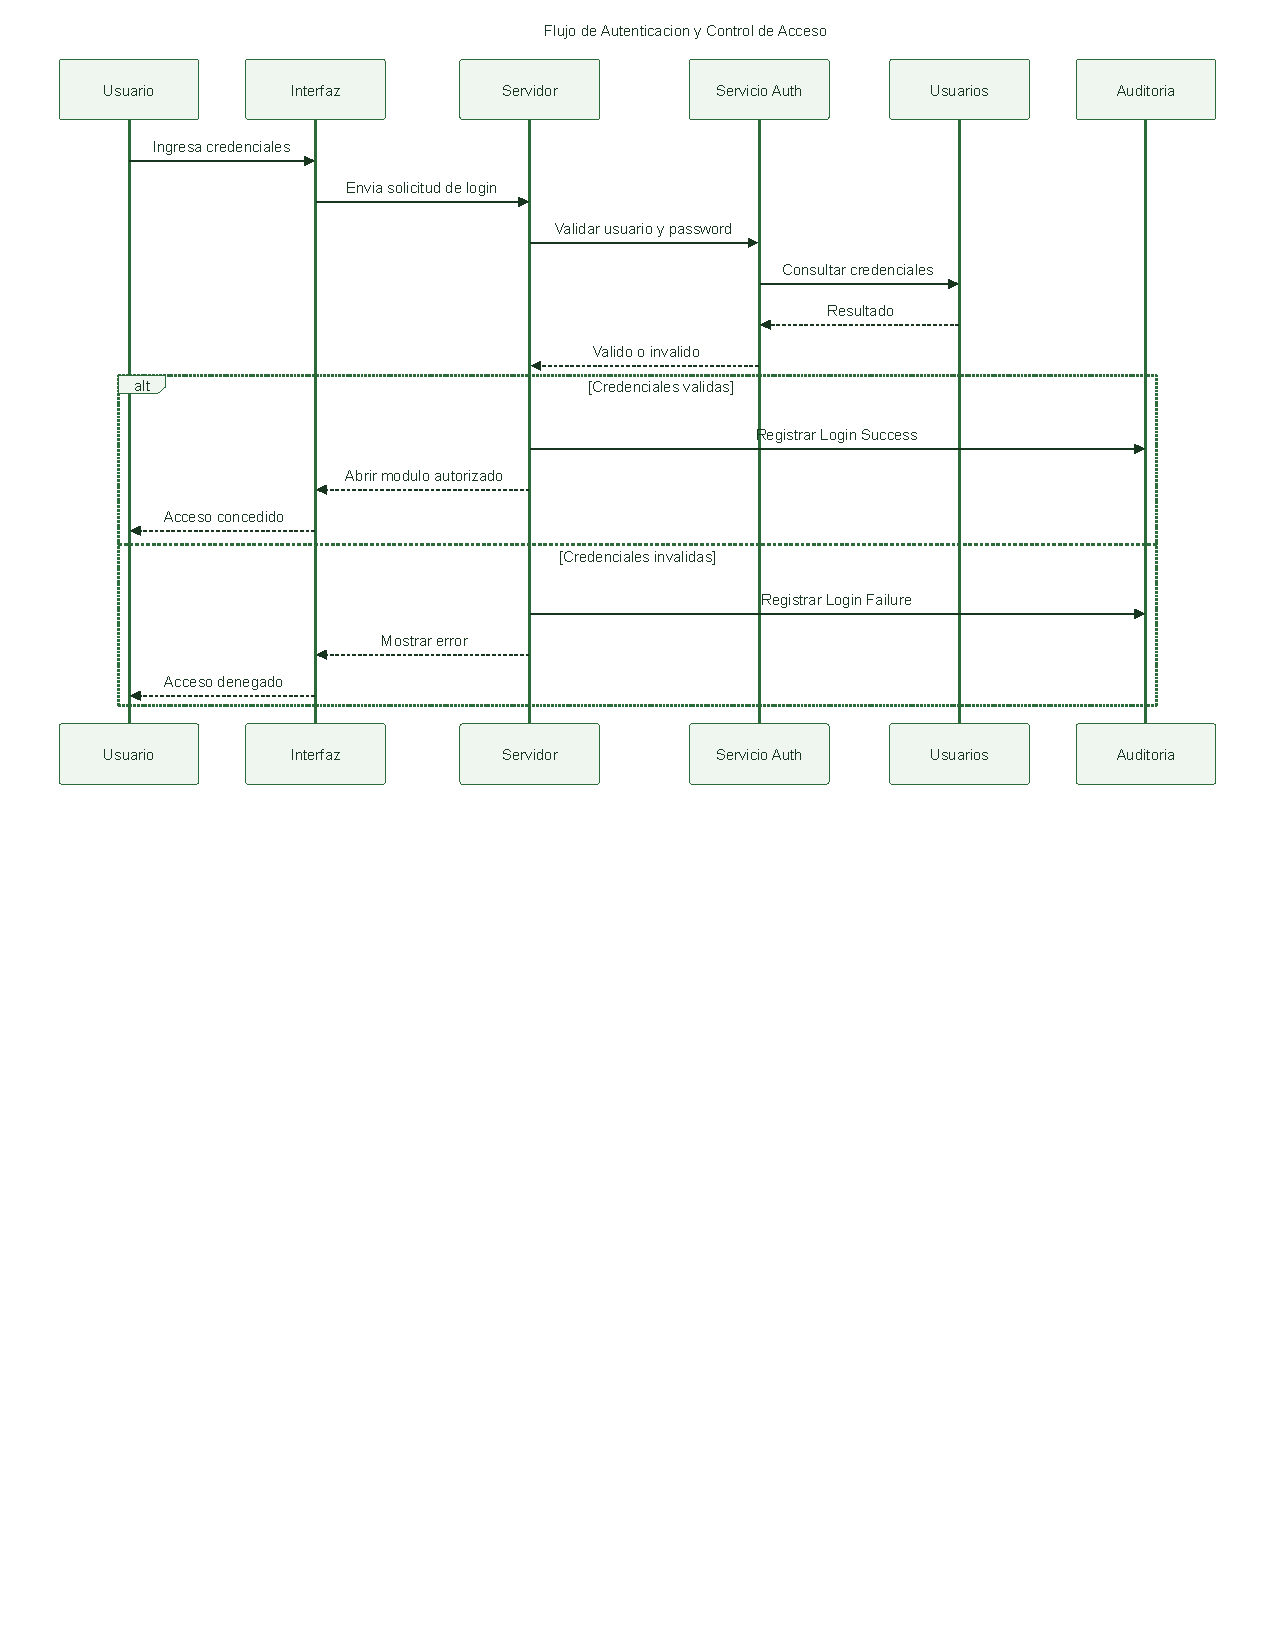
\includegraphics[width=0.95\textwidth]{figures/generated/02_flujo_autenticacion.pdf}
  \caption{Flujo de autenticacion y control de acceso}
  \label{fig:flujo-autenticacion}
\end{figure}
}{
\textit{Diagrama pendiente de exportacion: 02\_flujo\_autenticacion.pdf}
}

\section{Modelo de Datos}
La Figura~\ref{fig:modelo-datos} sintetiza el modelo de datos institucional y sus relaciones principales.
\IfFileExists{figures/generated/03_modelo_datos.pdf}{
\begin{figure}[htbp]
  \centering
  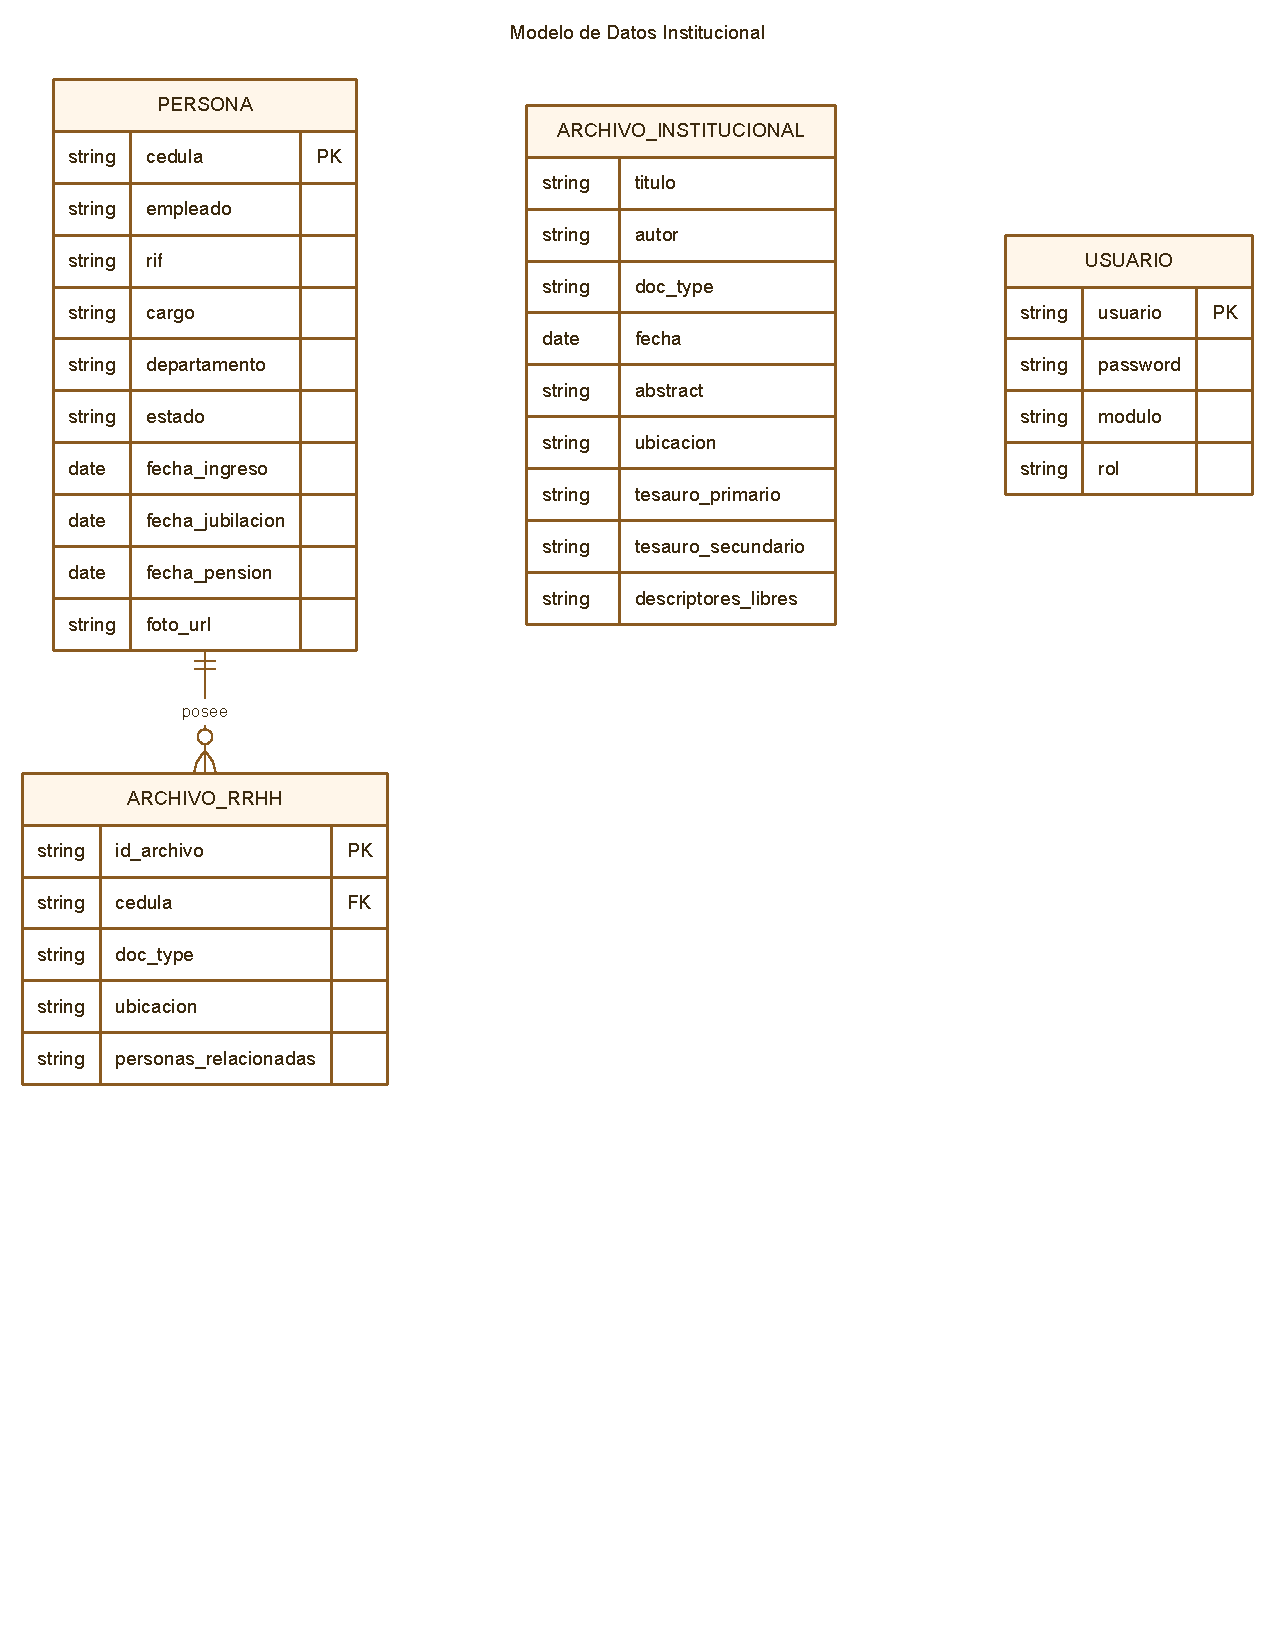
\includegraphics[width=\textwidth]{figures/generated/03_modelo_datos.pdf}
  \caption{Modelo de datos institucional}
  \label{fig:modelo-datos}
\end{figure}
}{
\textit{Diagrama pendiente de exportacion: 03\_modelo\_datos.pdf}
}

\section{Hoja de Ruta por Fases}
La Figura~\ref{fig:roadmap-fases} resume la progresión estratégica por fases y sus bloques de trabajo asociados.
\IfFileExists{figures/generated/04_roadmap_fases.pdf}{
\begin{figure}[htbp]
  \centering
  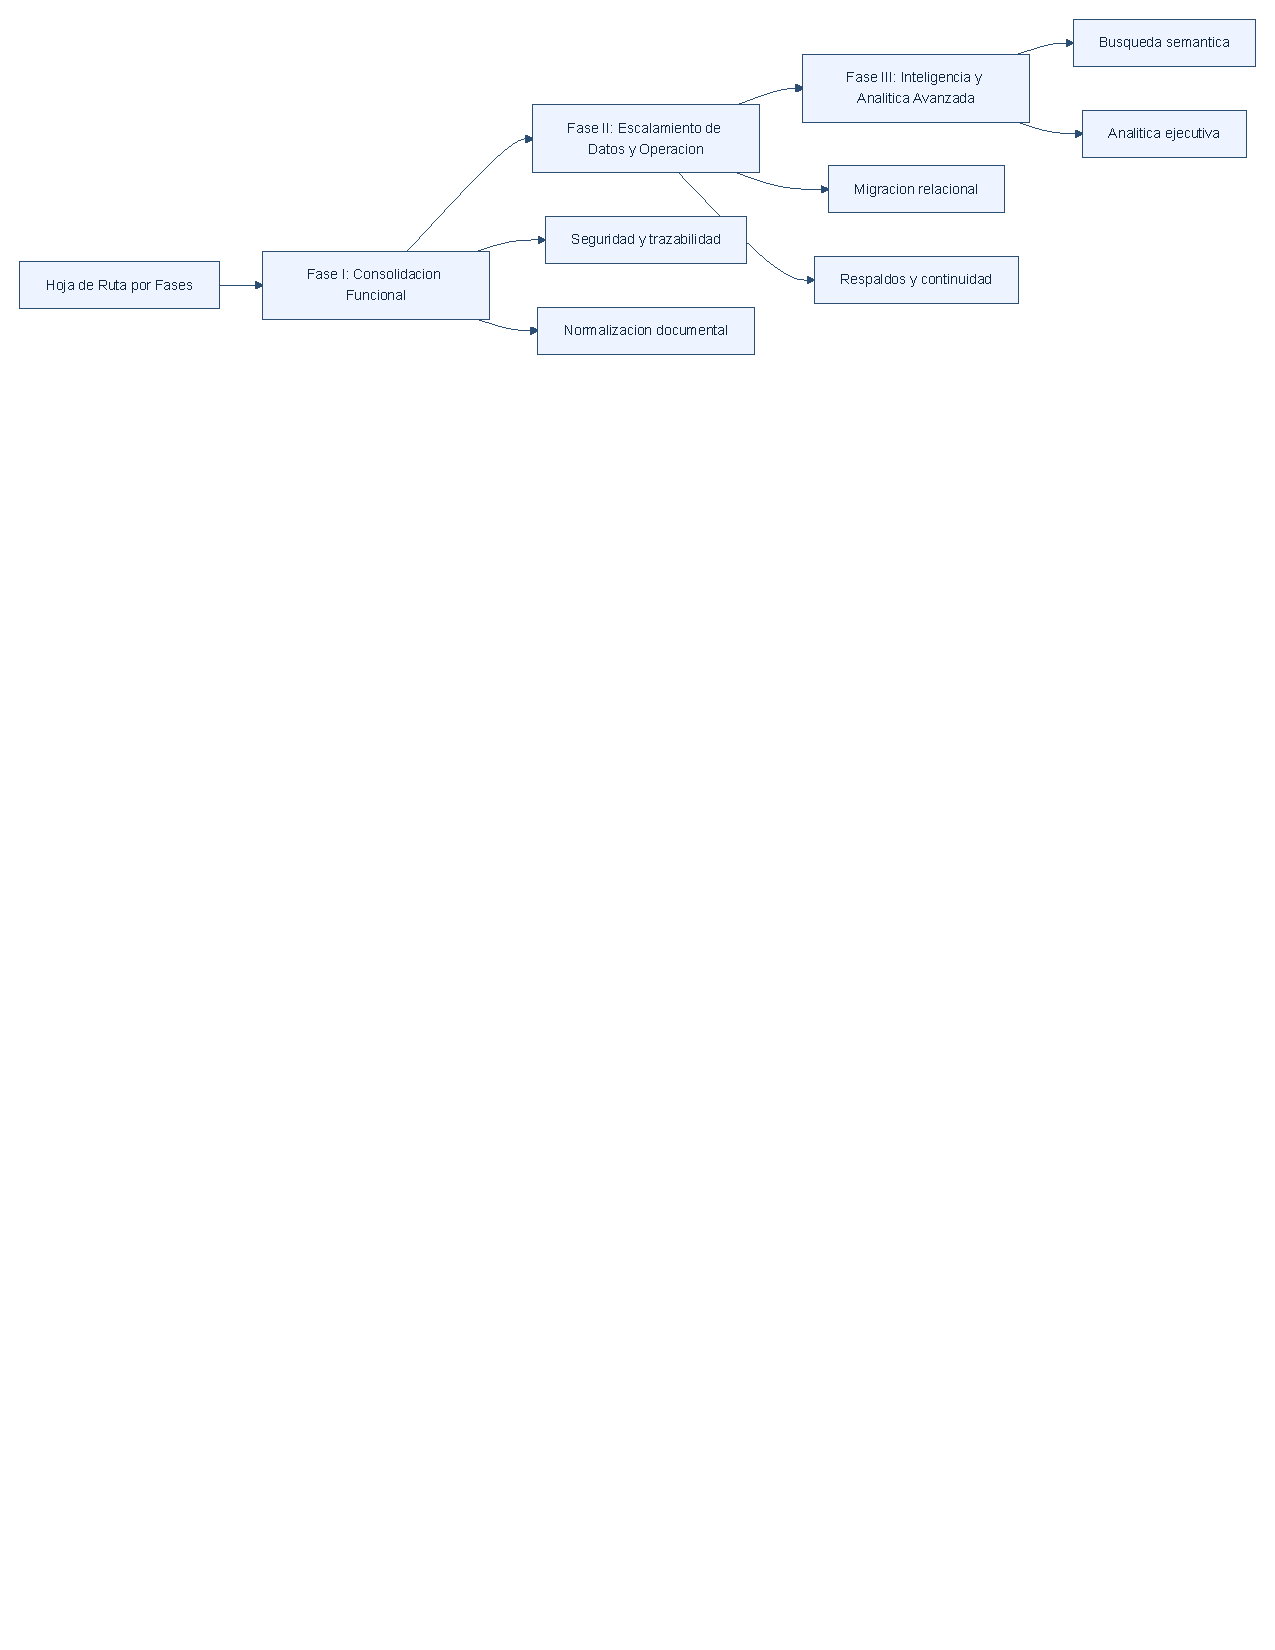
\includegraphics[width=\textwidth]{figures/generated/04_roadmap_fases.pdf}
  \caption{Hoja de ruta estrategica por fases}
  \label{fig:roadmap-fases}
\end{figure}
}{
\begin{figure}[htbp]
  \centering
  \begingroup
  \shorthandoff{<>}
  \begin{tikzpicture}[
    node distance = 1.0cm and 1.15cm,
    arr/.style={->, line width=0.9pt, >=Latex},
    stepA/.style={draw=blue!60!black, line width=0.9pt, rounded corners, minimum width=3.2cm, minimum height=0.95cm, font=\small, align=center, fill=blue!8},
    stepB/.style={draw=green!50!black, line width=0.9pt, rounded corners, minimum width=3.2cm, minimum height=0.95cm, font=\small, align=center, fill=green!8}
  ]
    \node[stepA] (f1) {Fase I\\Consolidacion Funcional};
    \node[stepA, right=of f1] (f2) {Fase II\\Escalamiento de Datos};
    \node[stepA, right=of f2] (f3) {Fase III\\Inteligencia y Analitica};

    \node[stepB, below=of f1] (h1) {Seguridad y Trazabilidad};
    \node[stepB, below=of f2] (h2) {Migracion Relacional};
    \node[stepB, below=of f3] (h3) {Busqueda Semantica};

    \draw[arr] (f1) -- (f2);
    \draw[arr] (f2) -- (f3);
    \draw[arr] (f1) -- (h1);
    \draw[arr] (f2) -- (h2);
    \draw[arr] (f3) -- (h3);
  \end{tikzpicture}
  \endgroup
  \caption{Hoja de ruta estrategica por fases (renderizado interno)}
  \label{fig:roadmap-fases}
\end{figure}
}

\section{Gobierno y Control de Acceso}
La Figura~\ref{fig:gobernanza-rbac} muestra cómo se articulan los comités, roles y módulos bajo el modelo de control de acceso.
\IfFileExists{figures/generated/05_gobernanza_rbac.pdf}{
\begin{figure}[htbp]
  \centering
  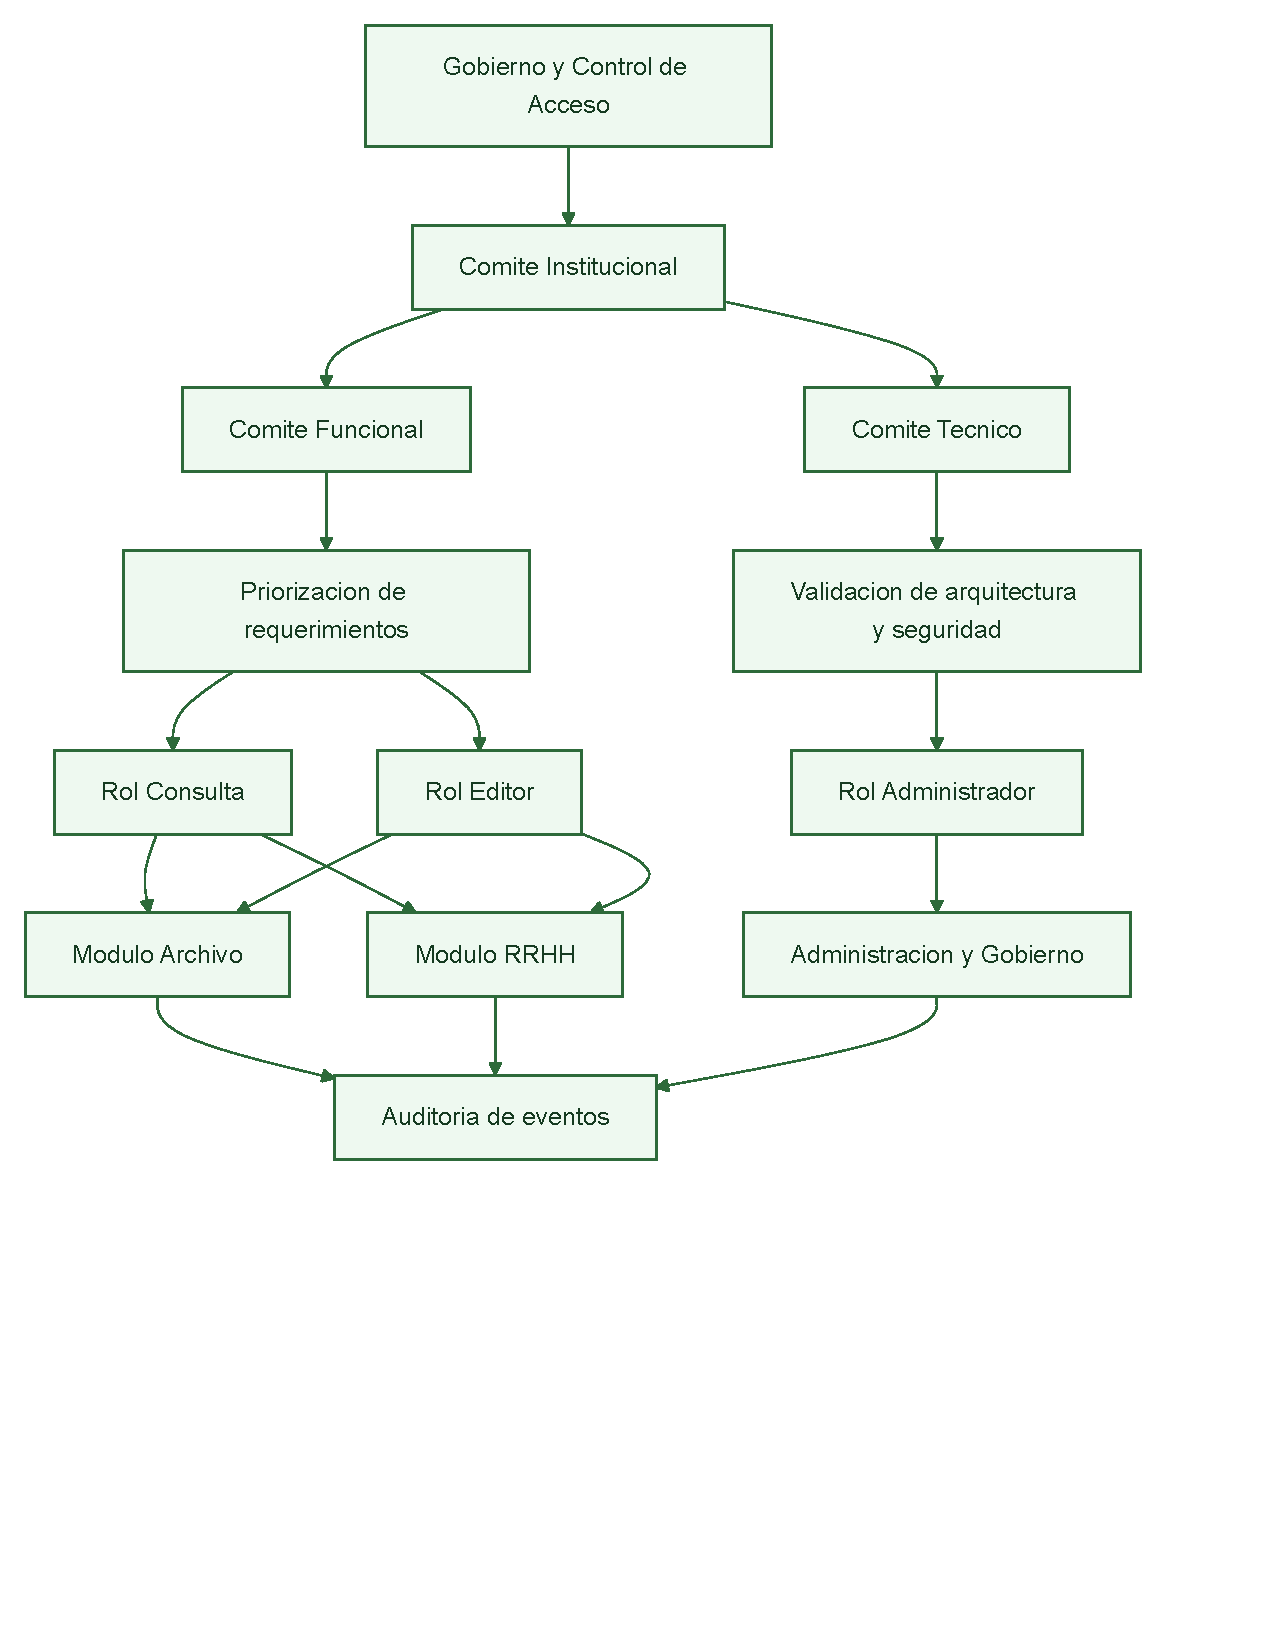
\includegraphics[width=\textwidth]{figures/generated/05_gobernanza_rbac.pdf}
  \caption{Gobierno funcional-tecnico y modelo de control de acceso}
  \label{fig:gobernanza-rbac}
\end{figure}
}{
\begin{figure}[htbp]
  \centering
  \begingroup
  \shorthandoff{<>}
  \begin{tikzpicture}[
    node distance = 1.0cm and 1.2cm,
    arr/.style={->, line width=0.9pt, >=Latex},
    gov/.style={draw=blue!60!black, line width=0.9pt, rounded corners, minimum width=3.2cm, minimum height=0.9cm, font=\small, align=center, fill=blue!8},
    rol/.style={draw=green!50!black, line width=0.9pt, rounded corners, minimum width=3.2cm, minimum height=0.9cm, font=\small, align=center, fill=green!8},
    dom/.style={draw=orange!70!black, line width=0.9pt, rounded corners, minimum width=3.2cm, minimum height=0.9cm, font=\small, align=center, fill=orange!10}
  ]
    \node[gov] (c) {Comite Institucional};
    \node[gov, below left=of c] (cf) {Comite Funcional};
    \node[gov, below right=of c] (ct) {Comite Tecnico};

    \node[rol, below=1.5cm of cf] (r1) {Rol Consulta};
    \node[rol, right=of r1] (r2) {Rol Editor};
    \node[rol, right=of r2] (r3) {Rol Administrador};

    \node[dom, below=1.5cm of r2] (a) {Modulo Archivo};
    \node[dom, left=of a] (h) {Modulo RRHH};
    \node[dom, right=of a] (g) {Administracion};
    \node[dom, below=of a] (log) {Auditoria de eventos};

    \draw[arr] (c) -- (cf);
    \draw[arr] (c) -- (ct);
    \draw[arr] (cf) -- (r1);
    \draw[arr] (cf) -- (r2);
    \draw[arr] (ct) -- (r3);
    \draw[arr] (r1) -- (a);
    \draw[arr] (r1) -- (h);
    \draw[arr] (r2) -- (a);
    \draw[arr] (r2) -- (h);
    \draw[arr] (r3) -- (g);
    \draw[arr] (a) -- (log);
    \draw[arr] (h) -- (log);
    \draw[arr] (g) -- (log);
  \end{tikzpicture}
  \endgroup
  \caption{Gobierno funcional-tecnico y modelo de control de acceso (renderizado interno)}
  \label{fig:gobernanza-rbac}
\end{figure}
}

\section{Despliegue y Continuidad Operativa}
La Figura~\ref{fig:despliegue-continuidad} ilustra el ciclo entre desarrollo, pruebas, producción, respaldo y recuperación.
\IfFileExists{figures/generated/06_despliegue_continuidad.pdf}{
\begin{figure}[htbp]
  \centering
  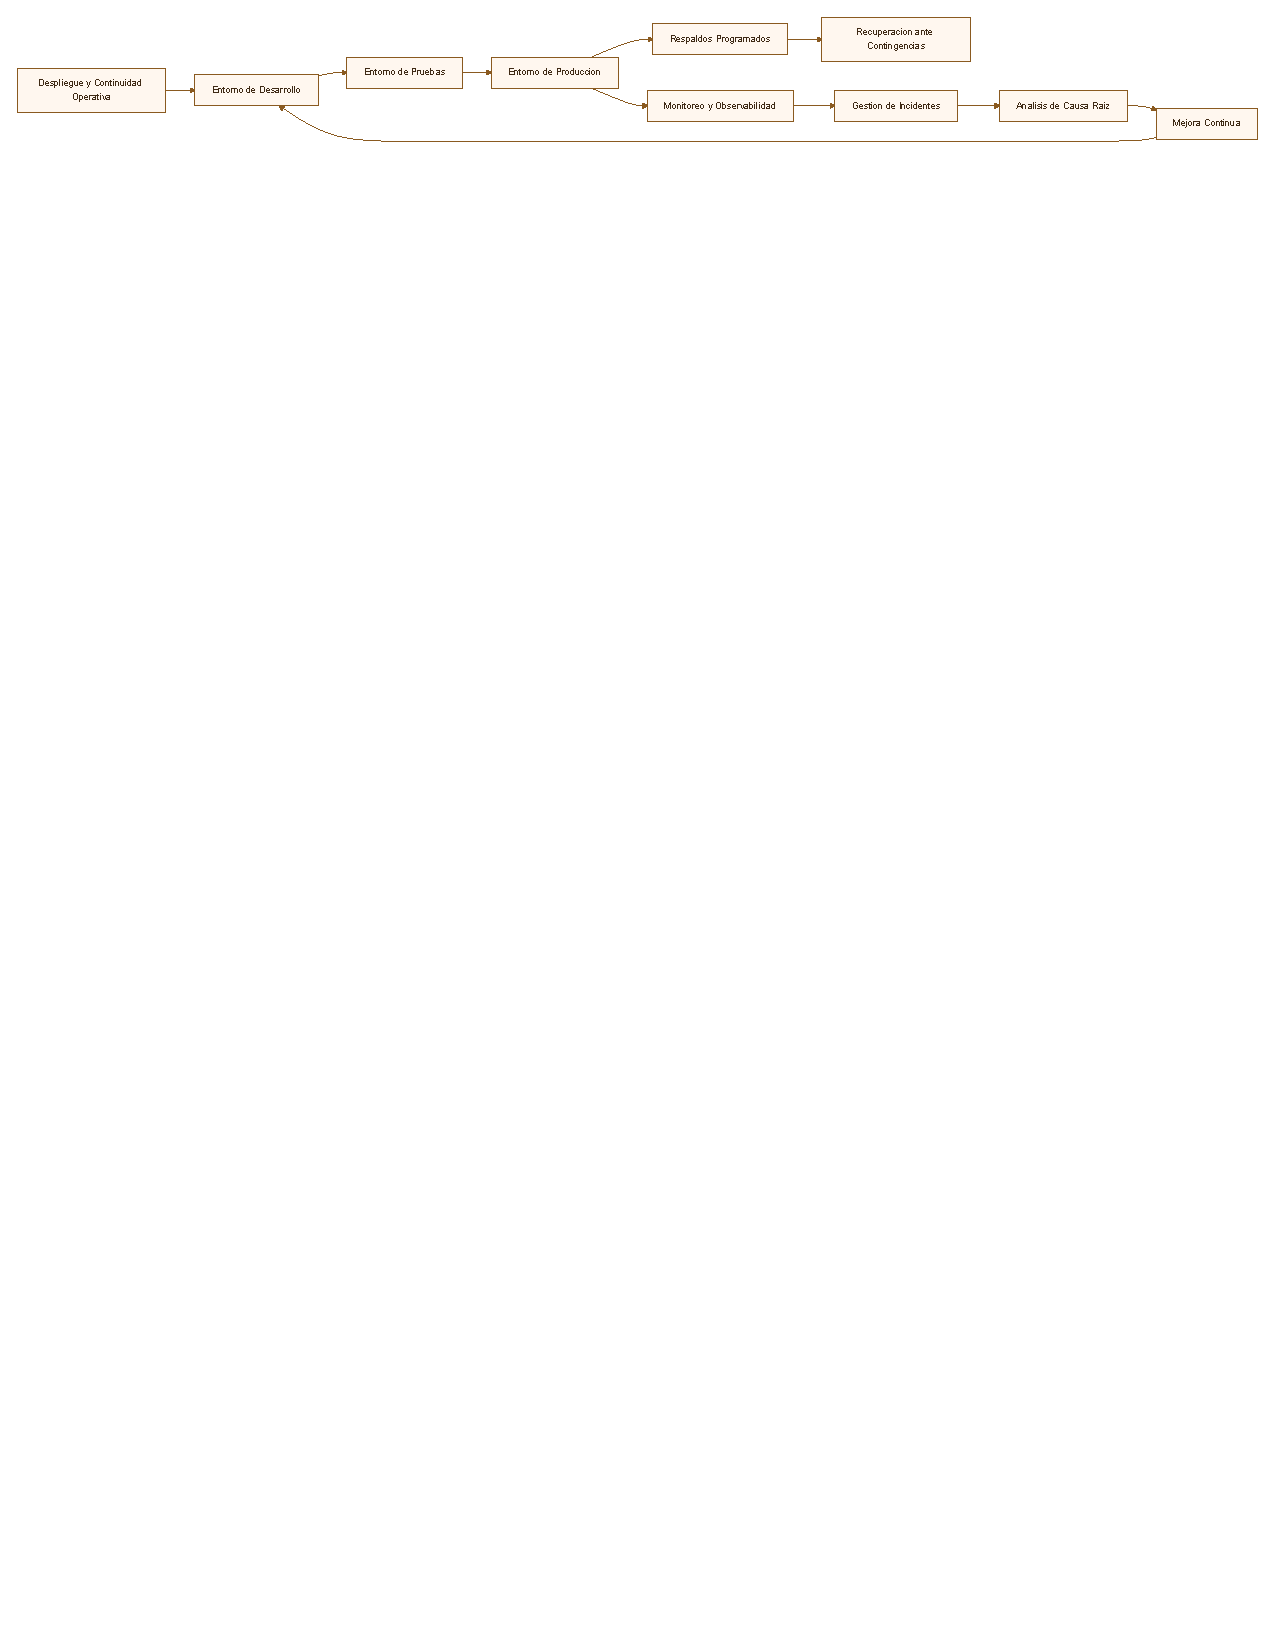
\includegraphics[width=\textwidth]{figures/generated/06_despliegue_continuidad.pdf}
  \caption{Ciclo de despliegue, respaldo y recuperacion operativa}
  \label{fig:despliegue-continuidad}
\end{figure}
}{
\begin{figure}[htbp]
  \centering
  \begingroup
  \shorthandoff{<>}
  \begin{tikzpicture}[
    node distance = 1.0cm and 1.1cm,
    arr/.style={->, line width=0.9pt, >=Latex},
    phase/.style={draw=blue!60!black, line width=0.9pt, rounded corners, minimum width=3cm, minimum height=0.9cm, font=\small, align=center, fill=blue!8},
    ops/.style={draw=green!50!black, line width=0.9pt, rounded corners, minimum width=3cm, minimum height=0.9cm, font=\small, align=center, fill=green!8},
    risk/.style={draw=orange!70!black, line width=0.9pt, rounded corners, minimum width=3cm, minimum height=0.9cm, font=\small, align=center, fill=orange!10}
  ]
    \node[phase] (d) {Desarrollo};
    \node[phase, right=of d] (t) {Pruebas};
    \node[phase, right=of t] (p) {Produccion};
    \node[ops, below=of p] (m) {Monitoreo};
    \node[ops, left=of m] (b) {Respaldos};
    \node[risk, below=of m] (r) {Recuperacion};
    \node[risk, left=of r] (i) {Incidentes y mejora};

    \draw[arr] (d) -- (t);
    \draw[arr] (t) -- (p);
    \draw[arr] (p) -- (m);
    \draw[arr] (p) -- (b);
    \draw[arr] (b) -- (r);
    \draw[arr] (m) -- (r);
    \draw[arr] (r) -- (i);
    \draw[arr] (i) |- (d);
  \end{tikzpicture}
  \endgroup
  \caption{Ciclo de despliegue, respaldo y recuperacion operativa (renderizado interno)}
  \label{fig:despliegue-continuidad}
\end{figure}
}

\section{Paquetes del Sistema}
La Figura~\ref{fig:paquetes-sistema} organiza las dependencias principales entre interfaz, núcleo, servicios, módulos y datos.
\IfFileExists{figures/generated/07_paquetes_sistema.pdf}{
\begin{figure}[htbp]
  \centering
  
\includegraphics[width=\textwidth]{figures/generated/07_paquetes_sistema.pdf}
  \caption{Diagrama de paquetes y dependencias principales del sistema}
  \label{fig:paquetes-sistema}
\end{figure}
}{
\begin{figure}[htbp]
  \centering
  \begingroup
  \shorthandoff{<>}
  \begin{tikzpicture}[
    node distance = 1.2cm and 1.3cm,
    arr/.style={->, line width=0.9pt, >=Latex},
    pA/.style={draw=blue!60!black, line width=0.9pt, rounded corners, align=center, minimum width=3.2cm, minimum height=0.9cm, font=\small, fill=blue!8},
    pB/.style={draw=green!50!black, line width=0.9pt, rounded corners, align=center, minimum width=3.2cm, minimum height=0.9cm, font=\small, fill=green!8},
    pC/.style={draw=orange!70!black, line width=0.9pt, rounded corners, align=center, minimum width=3.2cm, minimum height=0.9cm, font=\small, fill=orange!10}
  ]
    \node[pA] (ui) {Paquete UI\\ui.R + ui\_main\_body.R};
    \node[pA, right=of ui] (core) {Paquete Core\\app.R, global.R, server.R};
    \node[pB, below=of core] (svc) {Paquete Servicios\\auth, filters, persons, export, audit};
    \node[pB, left=of svc] (mod) {Paquete Modulos\\admin, stats, modal};
    \node[pC, right=of svc] (dat) {Paquete Datos\\usuarios, archivo, rrhh};

    \draw[arr] (ui) -- (core);
    \draw[arr] (core) -- (svc);
    \draw[arr] (core) -- (mod);
    \draw[arr] (mod) -- (svc);
    \draw[arr] (svc) -- (dat);
  \end{tikzpicture}
  \endgroup
  \caption{Diagrama de paquetes y dependencias principales del sistema (renderizado interno)}
  \label{fig:paquetes-sistema}
\end{figure}
}

\section{Casos de Uso Generales}
La Figura~\ref{fig:casos-uso-general} resume los actores y las acciones generales que cubre la aplicación.
\IfFileExists{figures/generated/08_casos_uso_general.pdf}{
\begin{figure}[htbp]
  \centering
  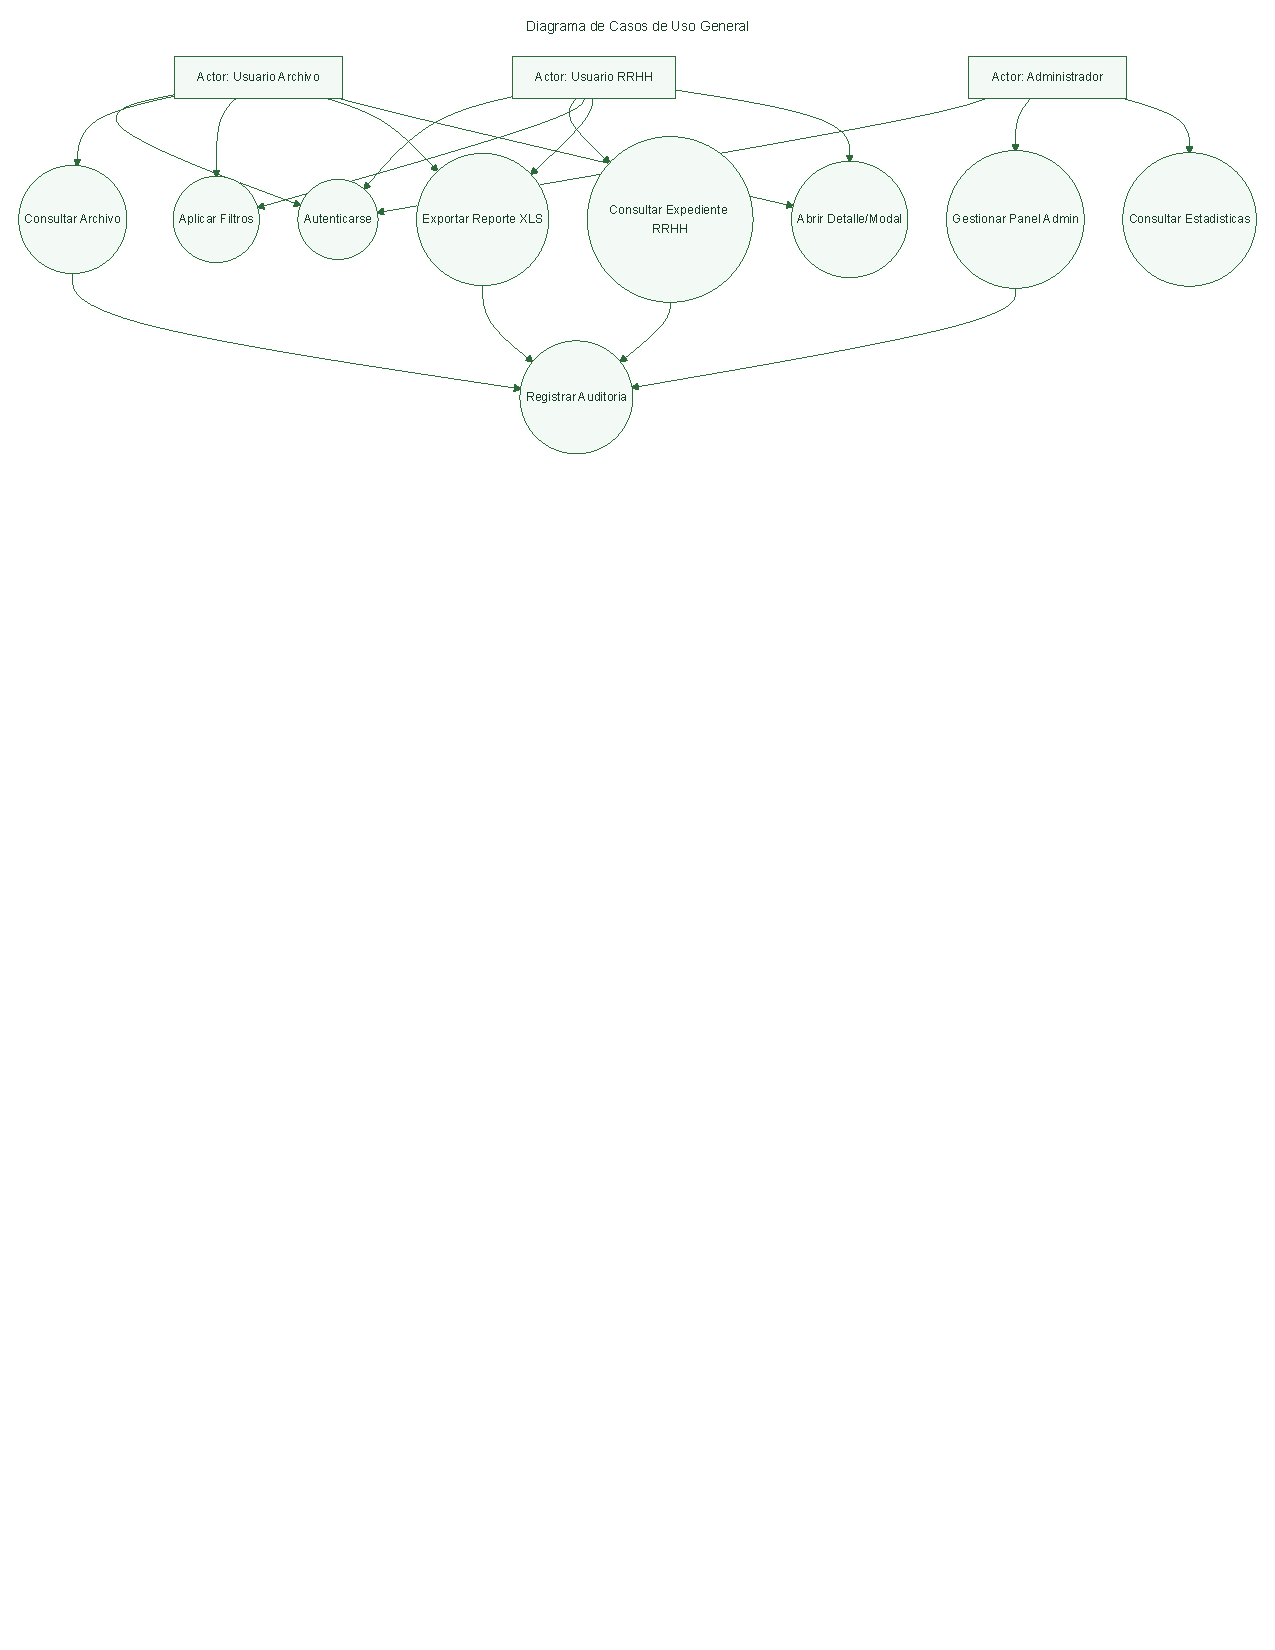
\includegraphics[width=\textwidth]{figures/generated/08_casos_uso_general.pdf}
  \caption{Vista general de actores y casos de uso del sistema}
  \label{fig:casos-uso-general}
\end{figure}
}{
\begin{figure}[htbp]
  \centering
  \begingroup
  \shorthandoff{<>}
  \begin{tikzpicture}[
    node distance = 1.1cm and 1.4cm,
    arr/.style={->, line width=0.9pt, >=Latex},
    actor/.style={draw=blue!60!black, line width=0.9pt, circle, minimum size=0.9cm, font=\small, align=center, fill=blue!8},
    usecase/.style={draw=green!50!black, line width=0.9pt, rounded corners, minimum width=3.2cm, minimum height=0.95cm, font=\small, align=center, fill=green!8}
  ]
    \node[actor] (a1) {Archivo};
    \node[actor, below=of a1] (a2) {RRHH};
    \node[actor, below=of a2] (a3) {Admin};

    \node[usecase, right=3.0cm of a1] (u1) {Autenticarse};
    \node[usecase, below=of u1] (u2) {Consultar Archivo};
    \node[usecase, below=of u2] (u3) {Consultar Expediente RRHH};
    \node[usecase, below=of u3] (u4) {Exportar Reporte XLS};
    \node[usecase, below=of u4] (u5) {Gestionar Panel Admin};

    \draw[arr] (a1) -- (u1);
    \draw[arr] (a1) -- (u2);
    \draw[arr] (a1) -- (u4);

    \draw[arr] (a2) -- (u1);
    \draw[arr] (a2) -- (u3);
    \draw[arr] (a2) -- (u4);

    \draw[arr] (a3) -- (u1);
    \draw[arr] (a3) -- (u5);
  \end{tikzpicture}
  \endgroup
  \caption{Vista general de actores y casos de uso del sistema (renderizado interno)}
  \label{fig:casos-uso-general}
\end{figure}
}

\section{Ciclo de Vida de Entrega}
La Figura~\ref{fig:ciclo-vida-entrega} muestra la secuencia de entrega, calidad y retroalimentación del sistema.
\IfFileExists{figures/generated/09_ciclo_vida_entrega.pdf}{
\begin{figure}[htbp]
  \centering
  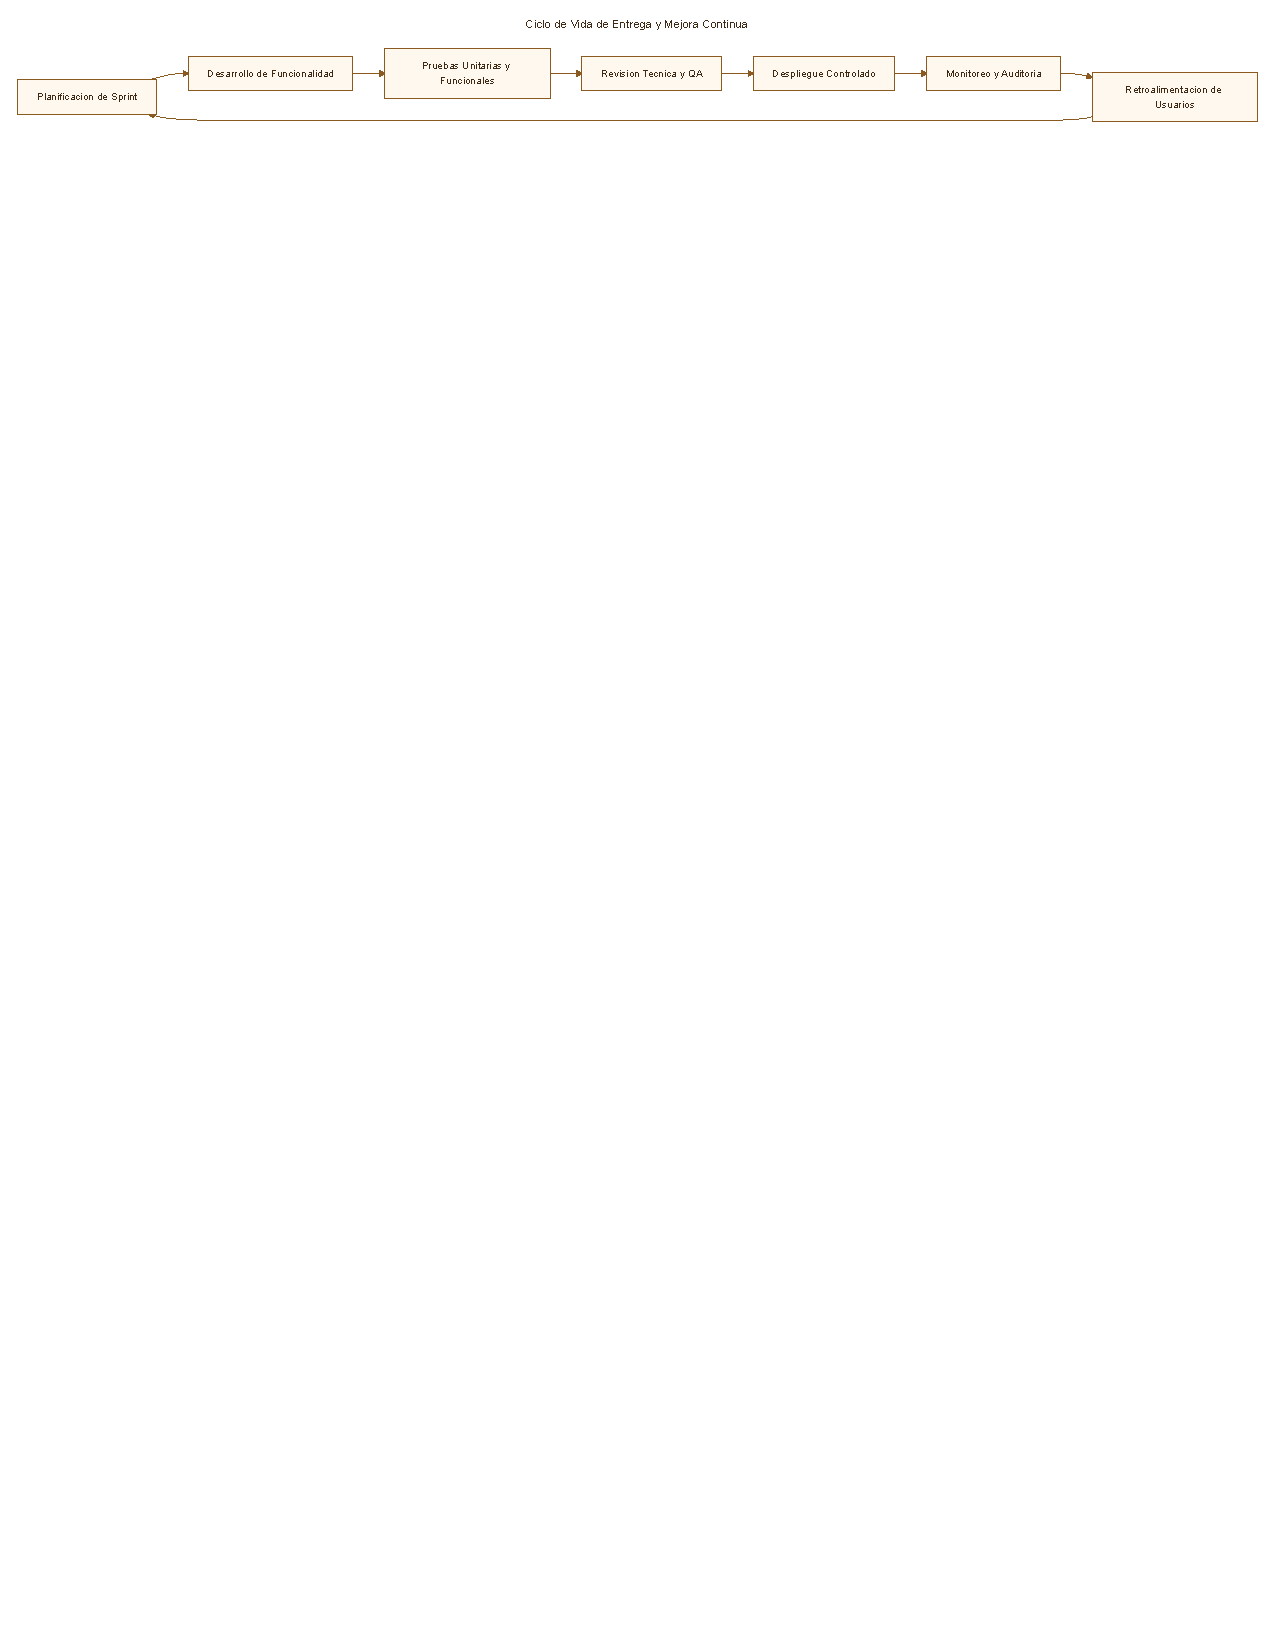
\includegraphics[width=\textwidth]{figures/generated/09_ciclo_vida_entrega.pdf}
  \caption{Ciclo de vida de entrega, control de calidad y mejora continua}
  \label{fig:ciclo-vida-entrega}
\end{figure}
}{
\begin{figure}[htbp]
  \centering
  \begingroup
  \shorthandoff{<>}
  \begin{tikzpicture}[
    node distance = 1.0cm and 1.2cm,
    arr/.style={->, line width=0.9pt, >=Latex},
    phase/.style={draw=blue!60!black, line width=0.9pt, rounded corners, minimum width=3.1cm, minimum height=0.9cm, font=\small, align=center, fill=blue!8},
    quality/.style={draw=green!50!black, line width=0.9pt, rounded corners, minimum width=3.1cm, minimum height=0.9cm, font=\small, align=center, fill=green!8},
    feedback/.style={draw=orange!70!black, line width=0.9pt, rounded corners, minimum width=3.1cm, minimum height=0.9cm, font=\small, align=center, fill=orange!10}
  ]
    \node[phase] (p1) {Planificacion};
    \node[phase, right=of p1] (p2) {Desarrollo};
    \node[quality, right=of p2] (p3) {Pruebas y QA};
    \node[quality, right=of p3] (p4) {Despliegue};
    \node[feedback, below=of p3] (p5) {Monitoreo y Auditoria};
    \node[feedback, left=of p5] (p6) {Retroalimentacion};

    \draw[arr] (p1) -- (p2);
    \draw[arr] (p2) -- (p3);
    \draw[arr] (p3) -- (p4);
    \draw[arr] (p4) |- (p5);
    \draw[arr] (p5) -- (p6);
    \draw[arr] (p6) |- (p1);
  \end{tikzpicture}
  \endgroup
  \caption{Ciclo de vida de entrega, control de calidad y mejora continua (renderizado interno)}
  \label{fig:ciclo-vida-entrega}
\end{figure}
}

